\documentclass{article}
\usepackage[utf8]{inputenc}
\usepackage[icelandic]{babel}
\usepackage[T1]{fontenc}
\usepackage{graphicx}
\usepackage{mathtools}
\usepackage{amsmath}
\usepackage{amssymb}
\usepackage{minted}


\graphicspath{ {./} }
\title{Verkleg æfing 2 - GHSR}
\author{ttb3@hi.is}
\date{\today}


\begin{document}
\maketitle


\section*{1. um hvað snérist verkefnið}
Verkefnið snérist um að útbúa kerfi sem hægt væri að nota í alvöru sem öryggiskerfi. Það hjálpar við að sýna
not fyrir sannleikstöflur og boolean algebru og notkun þeirra í raunheiminum. Maður þarf að breyta 'orðadæmi'
í rafrás í stað þess að fá annaðhvort gefið formúlu eða einhverskonar töflu.

\section*{2. hvað gerði ég}
Ég byrjaði á að skoða allt verkefnið og fá yfirlit yfir það. Síðan fylgdi ég hönnunarforsendunum eins og þær væru
uppskrift að mat og setti upp rarás í LogiSim, (cedar virkar ekki á linux). 
Fyrst bætti ég við öllum inntökum, gluggi 1 (g1), 
gluggi 2 (g2), útihurð (h), 
hreyfiskynjari 1 og 2 (s1,s2) og stöðubreyturnar kerfi er á (kerfi) og enginn er á staðnum (folk).
Í fyrsta drafti sameinaði ég g1, g2 og h sem einn rofa, s1 og s2 sem einn rofa, þá var ég bara með 4 input.
Fyrir fyrsta skilyrðið þurfti að athuga hvort kerfi sé 1, folk sé 1, og einhver af rofunum sé 1. Ég tengdi þá 
alla rofana saman í eitt OR hlið sem leiddi í AND hlið þar sem folk og kerfi tengdust líka.
Fyrir skilyrði 2 notaði ég sameinuðu g1, g2 og h og tengdi þá í AND hlið, í þetta AND hlið tengdust líka NOT folk og kerfi.
Bæði AND hliðin tengdust svo saman í OR hlið sem gaf öryggiskerfinu merki.
Þessi rás uppfyllir öll skilyrði en er ekki endilega sú einfaldasta en ég gerði mitt besta til þess að láta hana líta vel út.
\begin{center}
    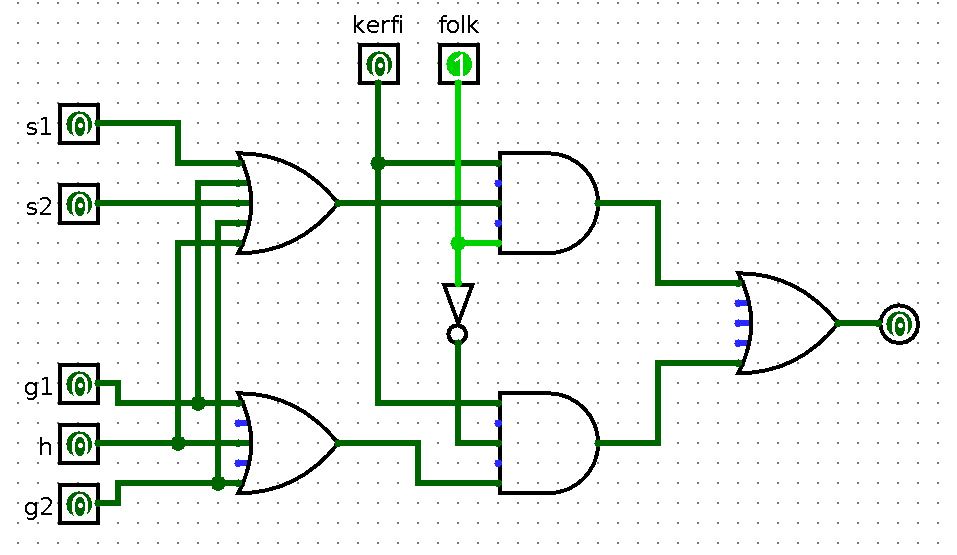
\includegraphics[scale=0.35]{ras.png}
\end{center}
Auðvelt væri að bæta við fleiri skynjurum, 
ef maður vill fá fleiri gluggaskynjara þarf bara að tengja í bæði skynjara og glugga OR hliðin. 
Að bæta við 'venjulegum' skynjara er einfaldara því þá þarf bara að bæti við skynjara OR hliðið.
Sjá næstu mynd, þar er búið að bæta við einum glugga og öðrum svæðisskynjara.
\begin{center}
    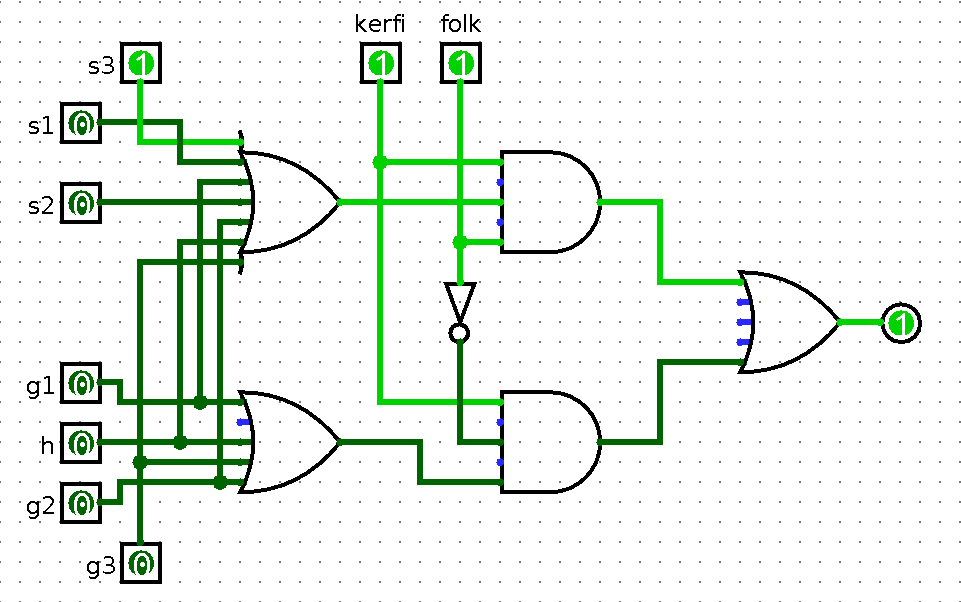
\includegraphics[scale=0.32]{rasVidbaett.png}
\end{center}

Boolean jafnan fyrir rásina, áður en hún er einfölduð, er auðvelt að lesa út 
$(folk*kerfi*(s1 + g1 + s2 + g2 + h)) + (kerfi*folk'*(g1 + g2))$, 
eftir að hún er einfölduð, þ.e. hurð og gluggar teknir saman í eina breytu GH, 
og svæðaskynjarar eru teknir saman í eina breytu S,\\
$(folk*kerfi*(S+GH)) + (folk'*kerfi*GH)$\\
Það að vera kominn með einfalda boolean jöfnu hjálpar mikið til við að búa til sanntöflu, hún lítur svona  út.
\begin{center}
    \begin{tabular}{|c|c|c|c|c|}
        \hline
        kerfi&folk&S&GH&out\\
        \hline
        0&0&0&0&0\\
        0&0&0&1&0\\
        0&0&1&0&0\\
        0&0&1&1&0\\
        0&1&0&0&0\\
        0&1&0&1&0\\
        0&1&1&0&0\\
        0&1&1&1&0\\
        1&0&0&0&0\\
        1&0&0&1&1\\
        1&0&1&0&0\\
        1&0&1&1&1\\
        1&1&0&0&0\\
        1&1&0&1&1\\
        1&1&1&0&1\\
        1&1&1&1&1\\
        \hline
    \end{tabular}
\end{center}

\section*{3. hvernig gekk}
verkefnið gekk bara vel, 
ég átti auðveldara að skilja þetta útfrá praktísku hliðinni en útfrá fræðilegu hliðinni og búa til rásina útfrá því.
Áhugavert að sjá hversu flókið kerfi er hægt að gera með einföldum rásum.

\section*{4. niðurstöður}
Boolean jafna, ekki einfölduð: $(folk*kerfi*(s1 + g1 + s2 + g2 + h)) + (kerfi*folk'*(g1 + g2))$\\
Boolean jafna, einfölduð: $(folk*kerfi*(S+GH)) + (folk'*kerfi*GH)$\\
Rásin:
\begin{center}
    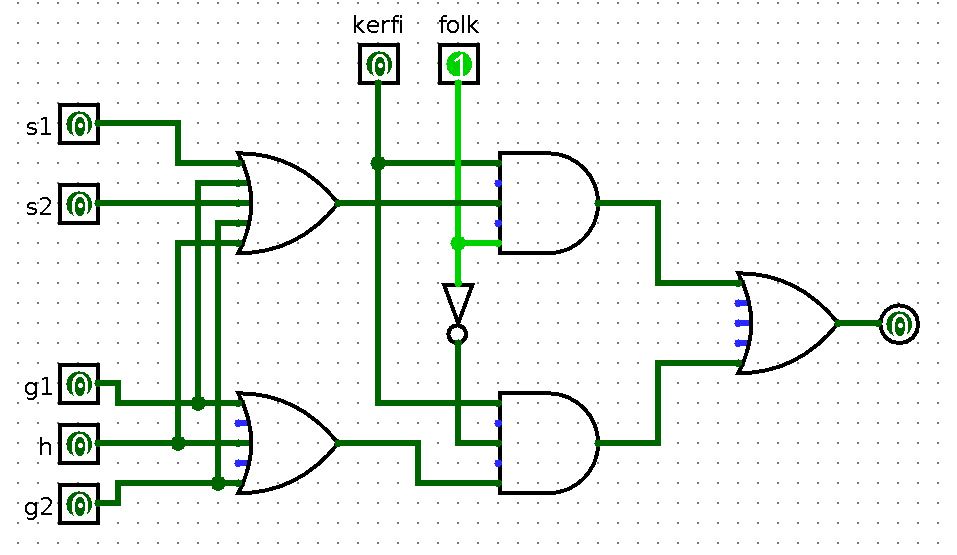
\includegraphics[scale=0.25]{ras.png}
\end{center}
\end{document}